\section{Point Spread Function}

\subsection{Définition et explication physique}

La fonction d'étalement du point (Point Spread Function), que l'on appelera dès maintenant la PSF, est une fonction qui décrit la réponse d'un système optique à un point lumineux (source ponctuelle). Dans notre cas, il s'agit de la réponse de l'optique de l'ELT à une étoile et son (ou ses) exoplanète(s).

Elle dépend de la longueur d'onde de la lumière observée, de la qualité de l'optique, de la turbulence atmosphérique, de la position de l'objet observé, etc. 

Pour calculer une PSF, on calcule la transformée de Fourier en deux dimensions de la pupille de l'instrument. La pupille est la surface d'entrée de la lumière dans l'instrument. La transformée de Fourier de la pupille donne la distribution de lumière dans le plan focal de l'instrument.

%Annexe du code ? en vrai c'est intéressant je pense


\subsection{La PSF de la pupille de L’ELT}

Prenons l'exemple de la PSF d'une étoile à travers la pupille de l'ELT.

% \begin{figure}[htbp]
%     \centering
%     
\includegraphics[width=0.35\textwidth]{figures/ELT_pupil.png}
%     \caption{Pupille de l'ELT. Les 6 araignées de l'ELT permettant de soutenir le miroir secondaire ainsi que le miroir secondaire y sont représenté. La partie blanche représentente les zones laissant passer la lumières. }
% \end{figure}

En calculant la PSF d'une étoile à travers cette pupille, on obtient une forme particulière, qui dépend de la longueur d'onde observée.

\begin{figure}[htbp]
    \centering
    \begin{subfigure}[b]{0.40\textwidth}
        \centering
        
\includegraphics[width=\textwidth]{figures/ELT_pupil.png}
        \caption{Pupille de l'ELT. }
    \end{subfigure}
    \hfill
    \begin{subfigure}[b]{0.46\textwidth}
        \centering
        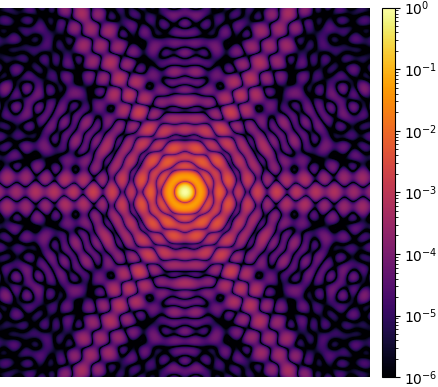
\includegraphics[width=\textwidth]{figures/PSF_ELT.png}
        \caption{PSF normalisé de l'ELT représenté en échelle logarithme.}
    \end{subfigure}
    \caption{\textit{None}}
\end{figure}

Sur la figure 6.1 on peut voir les 6 araignées de l'ELT permettant de soutenir le miroir secondaire ainsi que le miroir secondaire y sont représenté. La partie blanche représentente les zones laissant passer la lumières.

On normalise la PSF pour que l'intensité lumineuse soit maximale en son centre, et qu'on puisse voir l'image sous forme de contraste. Cela permet de mieux visualiser les zones où une exoplanète d'un certain contraste comparé à l'étoile serait potentiellement visible.

Ici, on obtient pas exactement une fonction de Bessel d'ordre 1, mais une forme similaire, avec un pic central et des anneaux de diffraction autour. Cette différence de forme est lié aux araignées de l'ELT, qui viennent perturber la propagation de la lumière ainsi que le miroir central.



\begin{figure}[htbp]
    \centering
    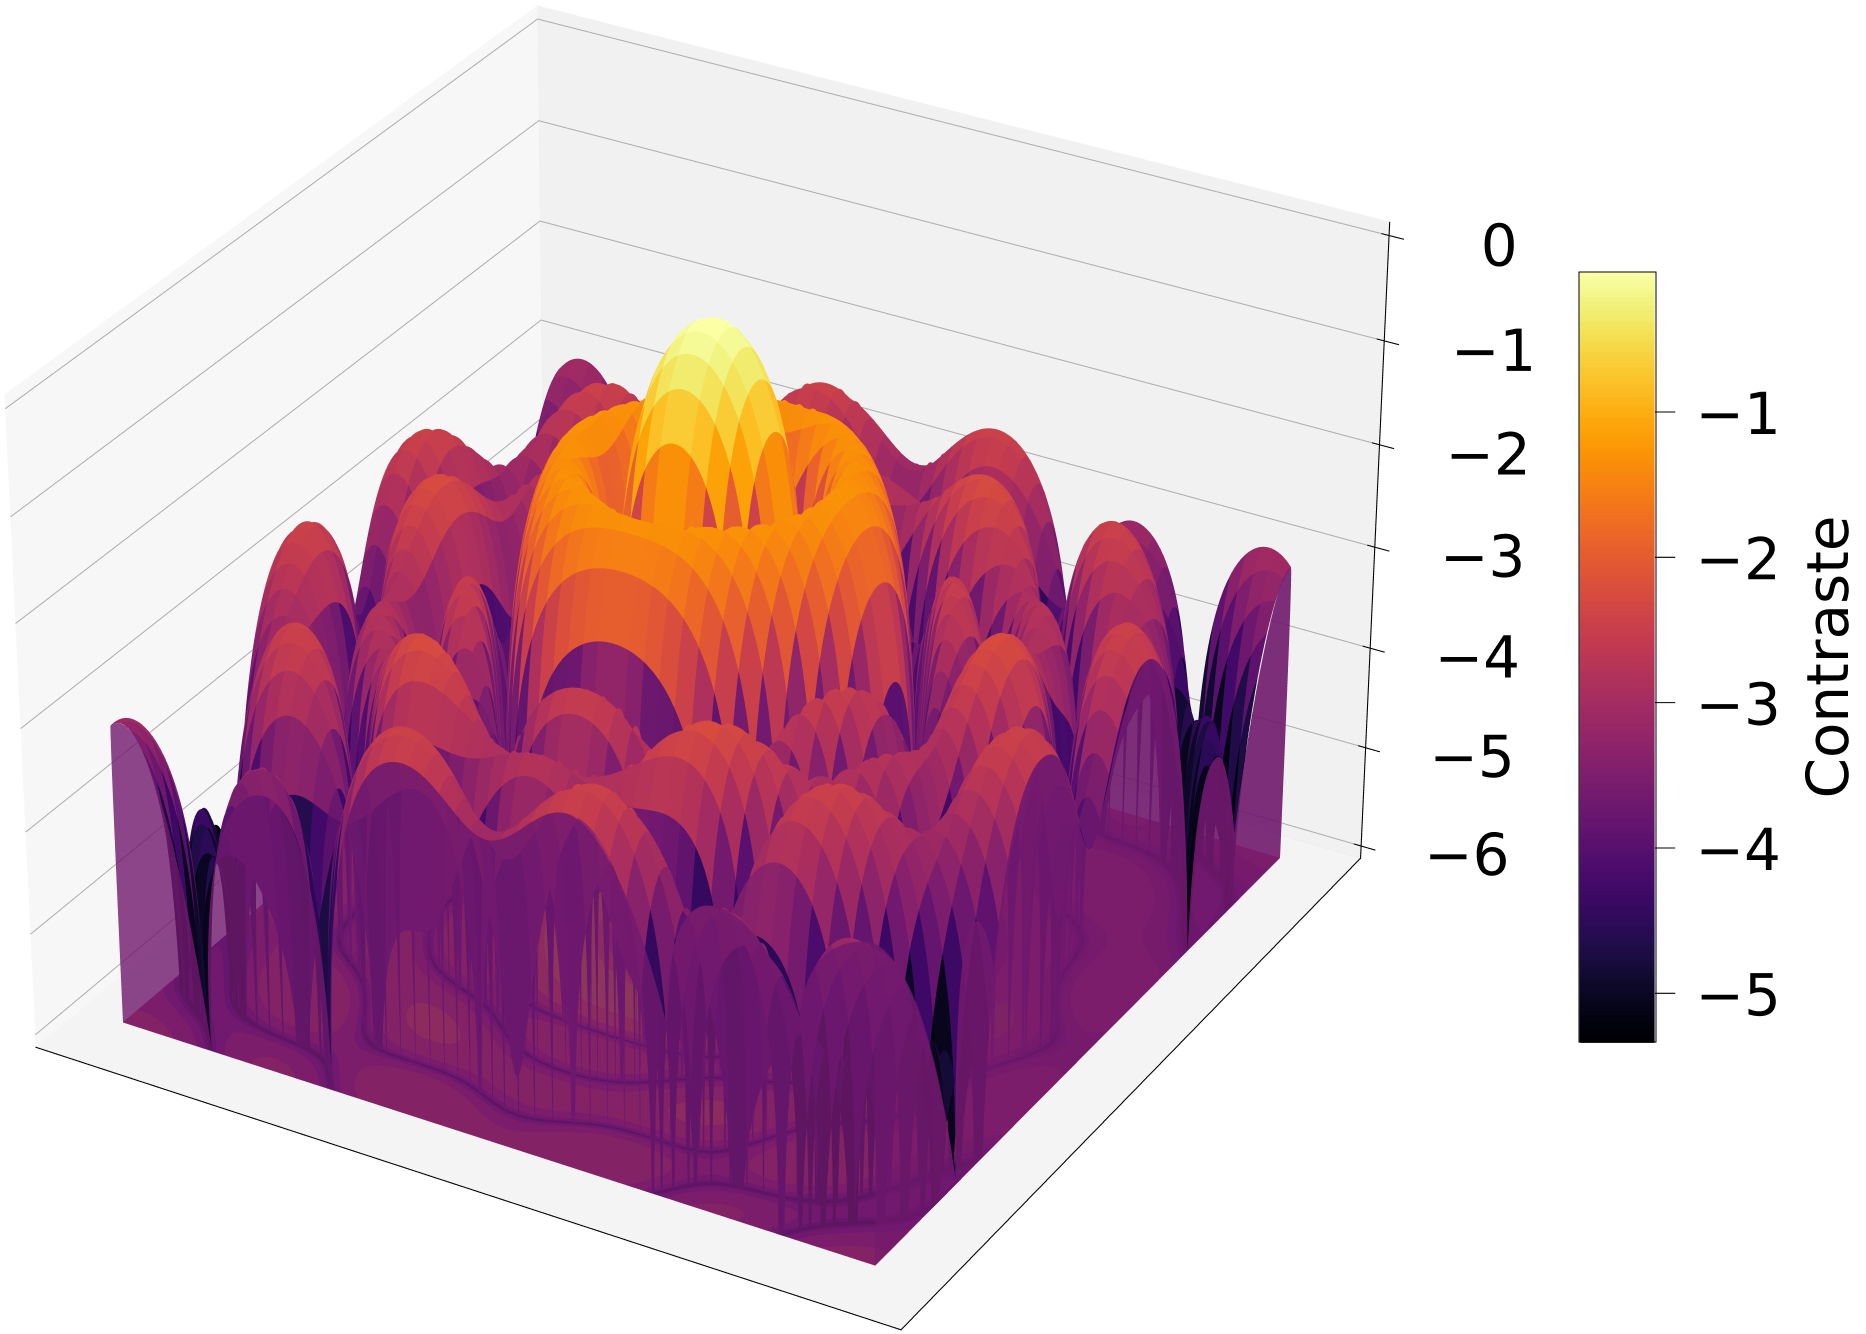
\includegraphics[width=0.7\textwidth]{figures/PSF_ELT_3D_bord.png}
    \caption{Représentation 3D de la PSF normalisé de l'ELT représenté en échelle logarithme. On peut voir les anneaux de diffraction autour du pic central.}
\end{figure}

Dans la fig7, on a zoomer sur les bords de la PSF pour mieux voir les anneaux de diffraction.

On se rend donc compte assez facilement de la difficulté de détecter la présence d'une exoplanète à faible séparation d'une étoile, car la PSF de l'étoile est très intense et très étendue, comparé au contraste de l'exoplanète qui sera trop faible.
%- rapidement la physique de comment on le calcule
%- expliqué c’est quoi une tache d’airy
- rapidement la physique et comment on le calcule dans le code


\subsection{Exemple avec un apodiseur d'HARMONI}

\begin{figure}[htbp]
    \centering
    % Première ligne avec SP1
    \begin{subfigure}[b]{0.40\textwidth}
        \centering
        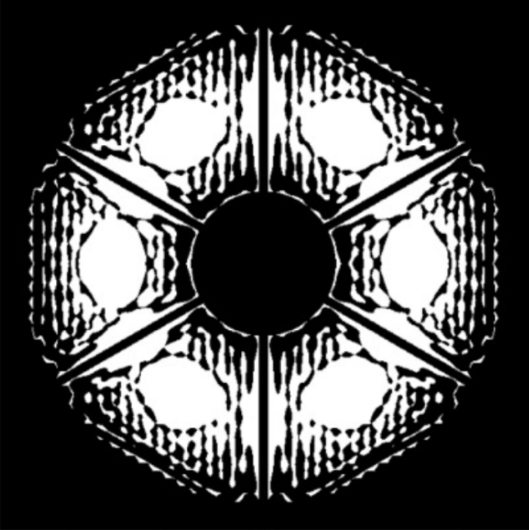
\includegraphics[width=\textwidth]{figures/SP1_HARMONI.png}
        \caption{Apodiseur SP1 de HARMONI-ELT.}
    \end{subfigure}
    \hfill % Espace entre les images
    \begin{subfigure}[b]{0.45\textwidth}
        \centering
        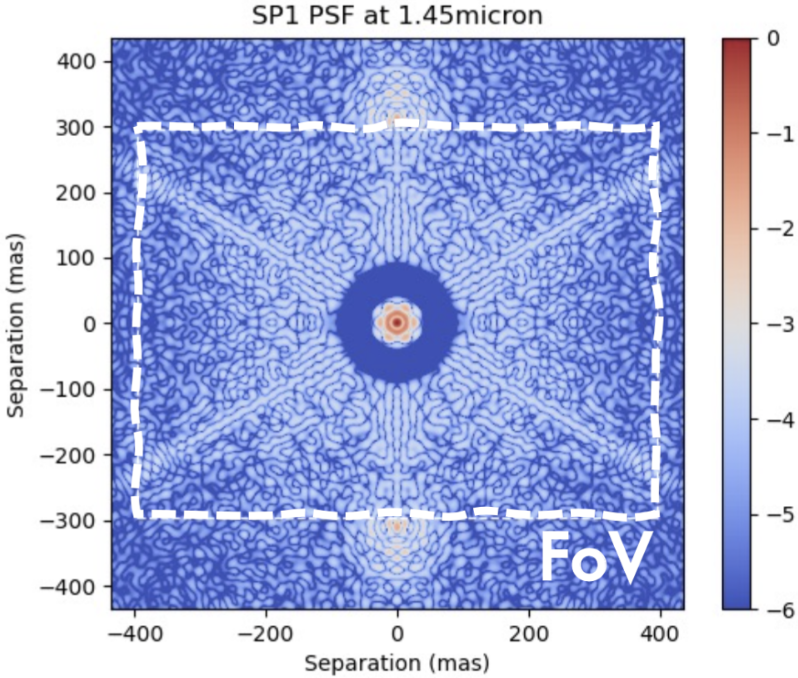
\includegraphics[width=\textwidth]{figures/PSF_SP1_HARMONI.png}
        \caption{PSF SP1 de HARMONI-ELT.}
    \end{subfigure}
    
    % Deuxième ligne avec SP2
    \begin{subfigure}[b]{0.40\textwidth}
        \centering
        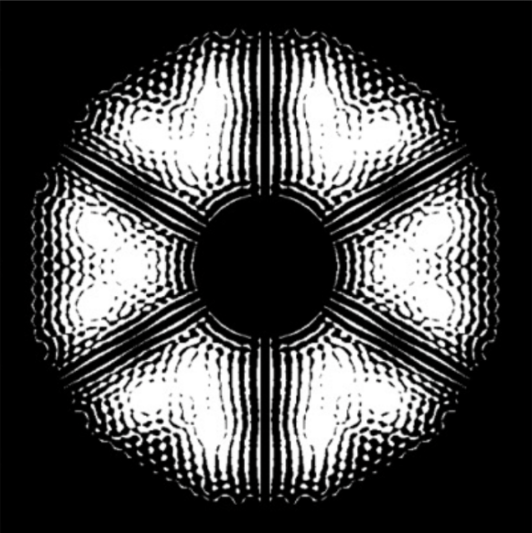
\includegraphics[width=\textwidth]{figures/SP2_HARMONI.png}
        \caption{Apodiseur SP2 de HARMONI-ELT.}
    \end{subfigure}
    \hfill % Espace entre les images
    \begin{subfigure}[b]{0.45\textwidth}
        \centering
        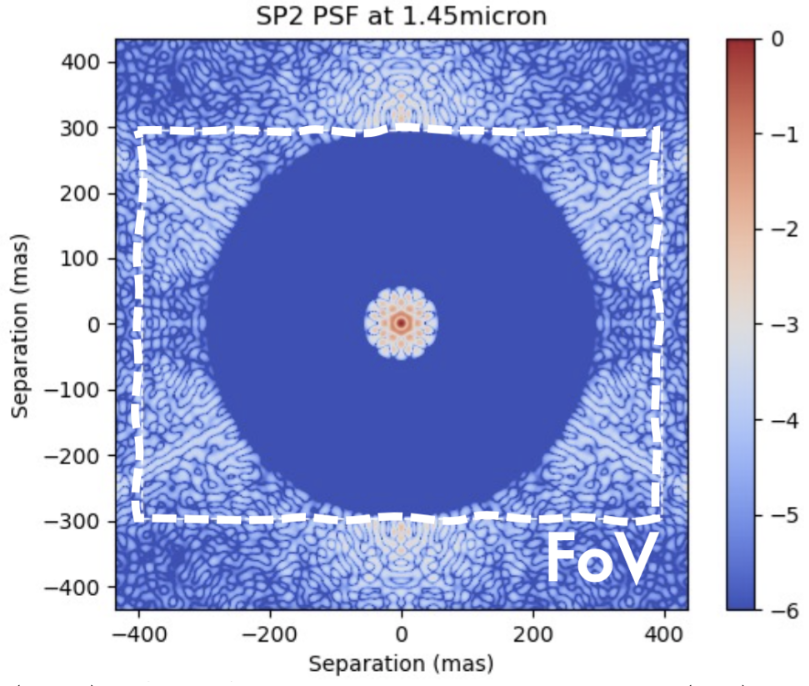
\includegraphics[width=\textwidth]{figures/PSF_SP2_HARMONI.png}
        \caption{PSF SP2 de HARMONI-ELT.}
    \end{subfigure}
    
    \caption{\textit{Comparaison des apodiseurs et des PSF pour SP1 et SP2 de HARMONI-ELT.}}
\end{figure}

\subsection{Nyquist}

On rappelle la définition de la fréquence de Nyquist : c'est la fréquence maximale que l'on peut observer dans un signal échantillonné. Elle est égale à la moitié de la fréquence d'échantillonnage.

Dans notre cas, cela signifie que pour observer correctement une planète, il faut que la planète soit échantillonnée par au moins 2 pixels par $\lambda/D$.

On présente 3 cas :
- On se trouve en dessous de Nyquist

Pas assez de données, on peut pas correctement analyser les données et affirmer ce qu'on voit (planète ou pas)

- On se trouve au dessus de Nyquist, on peut voir la planète
au moins 2 pixels par lambda/D

- On se trouve au dessus de Nyquist
temps de calcul trop long
- On se trouve à Nyquist

on peut voir la planète et analyser les données sans que ça prenne trop de temps de calcul

Mais que représente ces "temps de calcul" ? 
Il s'agit du calcul du SNR, que nous expliquons dans la section suivante.